\chapter{Bedingungen} \label{chp:Conditions}
\epigraph{In any moment of decision, the best thing you can do is the right thing, the next best thing is the wrong thing, and the worst thing you can do is nothing.}{Theodore Roosevelt}

Bis hierhin haben wir Programme mit \emph{linearem} Verlauf geschrieben: unsere Befehle werden von oben nach unten ohne Auslassungen oder Sprünge bearbeitet. Hier nun wollen wir erste Strukturen einführen, die den \emph{Programmfluss} ändern: Wir wollen bestimmte Code-Teile nur dann ausführen, wenn bestimmte \emph{Bedingungen} erfüllt sind.

\section{Wahrheitswerte} \label{sec:truthvalues}
Mathematischen Ausdrücken können \emph{Wahrheitswerte} zugeordnet werden. Diese Wahrheitswerte sagen aus, ob es sich um eine \enquote{wahre} oder \enquote{falsche} Aussage handelt. Ein Beispiel für einen solchen Ausdruck ist:
\begin{center}
\mintinline{c}{1 + 5 * 8 + 1 == 42}
\end{center}
Der Wahrheitswert dieses Ausdrucks ist offensichtlich \emph{wahr} (bzw. \emph{true}).

Beachten Sie bitte, dass für den \emph{Vergleich} zweier Zahlen das \emph{doppelte Gleichheitszeichen} \texttt{==} verwendet wird. Das einfache Gleichheitszeichen \texttt{=} dient ausschließlich der \emph{Wertzuweisung} an Variablen.

Tabelle \ref{tab:OperatorsComparison} listet Vergleichsoperatoren auf.
\begin{table}[h!]
	\newcolumntype{C}{>{         \centering\arraybackslash} p{.25\linewidth}}
	\newcolumntype{O}{>{\ttfamily\centering\arraybackslash} p{.20\linewidth}}
\begin{center}
\begin{tabularx}
	{.95\linewidth}
	{CO|CO}
\toprule[1pt]

	Vergleich           & \normalfont Zeichen  &
	Vergleich           & \normalfont Zeichen
\tabcrlf

	Gleichheit          & ==                   &  Ungleichheit         & != \\
	Kleiner als         & <                    &  Größer als           & >  \\
	Kleiner oder gleich & <=                   &  Größer oder gleich   & >= \\

\bottomrule[1pt]
\end{tabularx}
\end{center}
\caption{Vergleichsoperatoren in C}\label{tab:OperatorsComparison}
\end{table}

Da es nur zwei Wahrheitswerte gibt (\emph{wahr} und \emph{falsch}, bzw. \emph{true} und \emph{false}) wird im Prinzip nur ein einzelnes Bit benötigt, um einen solchen Wahrheitswert zu speichern. Ein Prozessor kann jedoch nur Gruppen zu mindestens 8 Bit behandeln, nicht aber einzelne Bits. Für uns sind Wahrheitswerte daher Ganzzahl-Werte, wie etwa \mintinline{c}{int}s. In der Tat lassen sich solche Wahrheitswerte speichern und ausgeben:

\begin{codebox}[Beispiel: Speichern und Ausgabe von Wahrheitswerten]
\begin{minted}[linenos]{c}
#include <stdio.h>

int main () {
   int    true   = 1 + 1 == 2,
          false  = 1 + 1 != 2;

   printf("Wert von 'true' : %d\n", true );
   printf("Wert von 'false': %d\n", false);
}
\end{minted}
\end{codebox}

Die Ausgabe hierzu lautet:

\begin{cmdbox}[Ausführungsbeispiel: Speichern und Ausgabe von Wahrheitswerten]
\begin{minted}{text}
Wert von 'true' : 1
Wert von 'false': 0
\end{minted}
\end{cmdbox}

Da eine \mintinline{c}{int}-Variable mehr Werte als \texttt{0} und \texttt{1} halten kann, interpretiert man alle von null verschiedenen Werte als \emph{wahr}.

Selbstverständlich können Ausdrücke, die zu Wahrheitswerten ausgewertet werden, auch Variablen enthalten. Es kann sogar mit ihnen gerechnet werden (auch wenn dies nur selten sinnvoll ist).

\begin{codebox}[Beispiel: Rechnen mit Wahrheitswerten]
\begin{minted}[linenos]{c}
#include <stdio.h>

int main () {
   int x     = 17,
       truth = (x > 5) + (x < 5) + (x == 17);

   printf("%d wahre Ausdrücke.\n", truth);
}
\end{minted}
\end{codebox}

\begin{cmdbox}[Ausführungsbeispiel: Rechnen mit Wahrheitswerten]
\begin{minted}{text}
2 wahre Ausdrücke.
\end{minted}
\end{cmdbox}

Nacheinander werden die drei Vergleiche \texttt{x > 5}, \texttt{x < 5} und \texttt{x == 17} ausgewertet (jeweils zu \texttt{1}, \texttt{0}, und \texttt{1}) und dann aufsummiert. Diese Summe wird in der normalen \mintinline{c}{int}-Variable \texttt{truth} gespeichert.

\begin{warnbox}[Symbole \texttt{true} und \texttt{false}]
Die Symbole \texttt{true} und \texttt{false} sind zwar nach keinem bisherigen C-Standard definiert; in vielen Bibliotheken sind diese Symbole aber mit den Werten \texttt{1} bzw. \texttt{0} definiert, und sollten daher auch ausschließlich im Sinne von Wahrheitswerten verwendet werden. Vermeiden Sie nach Möglichkeit die Verwendung der Symbole als Variablen ganz.

In C++ sind sowohl \mintinline{c++}{true} als auch \mintinline{c++}{false} fester Bestandteil der Sprache und können nicht als Variablennamen vergeben werden.
\end{warnbox}
\section{Bedingte Ausführung von Code: \mintinline{c}{if}}
Mit dem Konstrukt \mintinline{c}{if} lassen sich \emph{Wenn-Dann-Blöcke} erstellen: WENN \emph{Bedingung erfüllt}, DANN \emph{führe Anweisungen aus}. Bedingungen werden als mathematische Ausdrücke formuliert, die als erfüllt gelten, wenn ihr Wahrheitswert \emph{true} ist. \emph{Anweisungen} kann ein einzelner Befehl oder eine ganze Reihe von Befehlen sein. In der einfachsten Form sieht ein \mintinline{c}{if}-Block so aus:

\begin{codebox}[Syntax: Einfacher \texttt{if}-Block]
\begin{minted}{c}
if (Bedingung) {
   ... Anweisungen ...
}
\end{minted}
\end{codebox}

Im Kontext eines vollständigen Programms kann dies so aussehen:

\begin{codebox}[Beispiel: Einfacher \texttt{if}-Block]
\begin{minted}[linenos]{c}
#include <stdio.h>

int main () {
   int foo = 0;

   printf("Bitte geben Sie eine Ganzzahl ein:\n");
   scanf("%d", &foo);

   if (foo % 2 == 0) {
      printf("%d ist eine gerade Zahl.\n", foo);
   }

   printf("Sie haben %d eingegeben.\n", foo);
}
\end{minted}
\end{codebox}

Die Anweisung in Zeile 10 wird nur ausgeführt, wenn der Rest der Division von \texttt{foo} durch \texttt{2} gleich null ist, also wenn der Wert der Variablen gerade ist. Unabhängig vom Ausgang dieser Entscheidung wird Zeile 13 in jedem Fall ausgeführt.

Wenn auf die Bedingung nur eine einzelne Anweisung folgt (wie im obigen Beispiel), so können die \{geschweiften Klammern\} auch entfallen. Der folgende Code führt also zum selben Ergebnis:

\begin{codebox}[Beispiel: Einzeiliger \texttt{if}-Block]
\begin{minted}[linenos]{c}
#include <stdio.h>

int main () {
  int foo = 0;
  printf("Bitte geben Sie eine Ganzzahl ein:\n");
  scanf("%d", &foo);

  if (foo % 2 == 0)
    printf("%d ist eine gerade Zahl.\n", foo);

  printf("Sie haben %d eingegeben.\n", foo);
}
\end{minted}
\end{codebox}

\begin{warnbox}[Fehlerquelle fehlende Klammern]
Es mag praktisch erscheinen, die geschweiften Klammern bei einzeiligen \mintinline{c}{if}-Blocks nicht zu setzen. Nicht selten ergänzt man sein Programm im Laufe eines Projekts aber noch. Hängt man neue Befehle an einen \mintinline{c}{if}-Block an, so muss man diese Klammern natürlich nachsetzen. Dies wird oft vergessen. Betrachten Sie folgenden Code:

\begin{warnbox}[Beispiel: Fehlerhafter \texttt{if}-Block durch fehlende Klammern, leftupper=7mm]
\begin{minted}[linenos]{c}
#include <stdio.h>

int main () {
   int foo = 0;

   printf("Bitte geben Sie eine Ganzzahl ein:\n");
   scanf("%d", &foo);

   if (foo % 2 == 0)
      printf("%d ist eine gerade Zahl.\n", foo);
      printf("%d ist durch 2 teilbar.\n", foo);

   printf("Sie haben %d eingegeben.\n", foo);
}
\end{minted}
\end{warnbox}

Die Ausgabe in Zeile 10 findet nur statt, wenn \texttt{foo} einen geraden Wert hält; Zeile 11 dagegen wird fälschlicherweise \emph{immer} ausgeführt. Die Code-Einrückung -- eigentlich ein Zeichen guten Stils -- kaschiert diesen Fehler noch mehr. Ich rate daher dazu, \emph{immer} Klammern zu setzen. Richtig müsste der \mintinline{c}{if}-Block also lauten:

\begin{codebox}[Beispiel: Korrekter mehrzeiliger \texttt{if}-Block]
\begin{minted}[linenos,firstnumber=9]{c}
   if (foo % 2 == 0) {
      printf("%d ist eine gerade Zahl.\n", foo);
      printf("%d ist durch 2 teilbar.\n", foo);
   }
\end{minted}
\end{codebox}
\end{warnbox}

Mit dem Schlüsselwort \mintinline{c}{else} kann der \mintinline{c}{if}-Block noch um Anweisungen ergänzt werden, die nur ausgeführt werden sollen, wenn die Bedingung gerade \emph{nicht} erfüllt war:

\begin{codebox}[Beispiel: \texttt{if-else}-Block]
\begin{minted}[linenos]{c}
#include <stdio.h>

int main () {
  int foo = 0;
  printf("Bitte geben Sie eine Ganzzahl ein:\n");
  scanf("%d", &foo);
}
\end{minted}
\end{codebox}
%
\begin{codebox}[]
\begin{minted}[linenos, firstnumber=last]{c}
  if (foo % 2 == 0) {
    printf("%d ist eine gerade Zahl.\n", foo);
  } else {
    printf("%d ist eine ungerade Zahl.\n", foo);
  }
}
\end{minted}
\end{codebox}

\begin{hintbox}[Stil: Einrückungen und Position der Klammern]
Gute Programmierer sind sich einig, dass Einrückungen fester Bestandteil von gutem Code sind. Ohne diese verliert man in auch nur wenig komplexen Projekten schnell den Überblick und macht unnötige Fehler. Hier aber endet auch schon die Einigkeit; es gibt keine allgemein anerkannte \enquote{richtige Art, Code einzurücken}. Tabulatoren oder Leerzeichen, zwei oder vier Zeichen pro Einrückung, oder auch die Position der Klammern -- verschiedenste Varianten werden gelebt und kontrovers und teilweise sehr emotional diskutiert, wie Abbildung \ref{fig:IndentStyle} zeigt.

Sie sind also frei, Ihren Stil selbst zu definieren, sollten dabei aber zwei Regeln einhalten:
\begin{itemize}
\item Halten Sie Ihren Code einheitlich, \ie behalten Sie den Einrückungs-Stil über ein gesamtes Projekt konsistent.
\item Ändern Sie niemals den Einrückungs-Stil ihrer KollegInnen.
\end{itemize}
\end{hintbox}

\begin{figure}
	\href{http://www.sandraandwoo.com/2015/04/13/0674-there-are-10-types-of-programmers/}{
		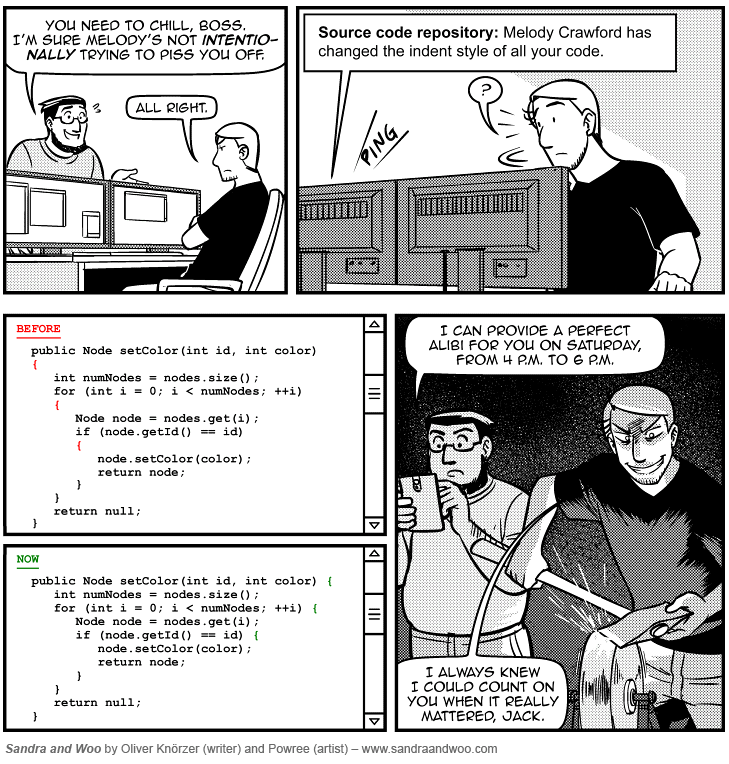
\includegraphics[width=\linewidth]{./gfx/SW-indent-style}
	}
	\caption{Ein realistisches Szenario} \label{fig:IndentStyle}
\end{figure}

\mintinline{c}{if}-Blöcke dürfen nahezu beliebig tief verschachtelt werden\footnote{Der Standard aus dem Jahre 1999 verpflichtet die Programmierer von C-Compilern zwar \enquote{nur} dazu, mindestens 127 Ebenen (256 für C++) zu unterstützen; im Falle des gcc bricht der Kompiliervorgang aber erst nach 6199 Ebenen mit Fehlermeldung ab.}. Das folgende Beispiel prüft also zuerst, ob eine eingegebene Zahl positiv war, und nur für positive Zahlen die \emph{Parität} (die Eigenschaft, gerade oder ungerade zu sein).

\begin{codebox}[Beispiel: Verschachtelter \texttt{if-else}-Block]
\begin{minted}[linenos]{c}
#include <stdio.h>

int main () {
   int foo = 0;

   printf("Bitte geben Sie eine Ganzzahl ein:\n");
   scanf("%d", &foo);

   if (foo > 0) {
      if (foo % 2 == 0) {
         printf("%d ist eine gerade Zahl.\n"  , foo);
      } else {
         printf("%d ist eine ungerade Zahl.\n", foo);
      }
   } else {
      printf("%d ist eine ungültige Zahl.\n"  , foo);
   }
}
\end{minted}
\end{codebox}

Spätestens an diesem Beispiel erkennen Sie, weshalb auf Einrückung so viel Wert gelegt wird. Sehen Sie sich zum Vergleich auch das folgende -- syntaktisch korrekte -- Beispiel ohne Einrückungen an:

\begin{warnbox}[Schlechter Stil: Code mit mehreren Hierarchie-Ebenen ohne Einrückungen, leftupper=7mm]
\begin{minted}[linenos]{c}
#include <stdio.h>
int main () {
int foo = 0;
printf("Bitte geben Sie eine Ganzzahl ein:\n");
scanf("%d", &foo);
if (foo > 0) {
if (foo % 2 == 0) {
printf("%d ist eine gerade Zahl.\n", foo);
} else {
printf("%d ist eine ungerade Zahl.\n", foo);
}} else {
printf("%d ist eine ungültige Zahl.\n", foo);
}}
\end{minted}
\end{warnbox}

Verschachtelte \mintinline{c}{if}-\mintinline{c}{else}-Blocks lassen sich formell auch auf einer Hierarchie-Ebene darstellen. Der folgende Code erzeugt dasselbe Verhalten wie die beiden obigen Beispiele, wirkt aber in manchen Augen klarer\footnote{Technisch handelt es sich hierbei um eine Anwendung der Regel, dass bei einzeiligen \mintinline{c}{if}-Blocks die Klammern entfallen können.}:

\begin{codebox}[Beispiel: \texttt{if}-Block mit mehreren Fällen]
\begin{minted}[linenos]{c}
#include <stdio.h>

int main () {
   int foo = 0;

   printf("Bitte geben Sie eine Ganzzahl ein:\n");
   scanf("%d", &foo);

   if        (foo <= 0) {
      printf("%d ist eine ungültige Zahl.\n", foo);
   } else if (foo % 2 == 0) {
      printf("%d ist eine gerade Zahl.\n"   , foo);
   } else {
      printf("%d ist eine ungerade Zahl.\n" , foo);
   }
}
\end{minted}
\end{codebox}

Achten Sie bei dieser Form aber darauf, dass nur der Code zur \emph{ersten erfüllten Bedingung} ausgeführt wird, selbst wenn nachfolgende Blocks ebenfalls den Wahrheitswert \emph{true} haben:

\begin{codebox}[Beispiel: \texttt{if}-Block mit unerreichbarem Code]
\begin{minted}[linenos]{c}
#include <stdio.h>

int main () {
   int foo = 0;

   printf("Bitte geben Sie eine Ganzzahl ein:\n");
   scanf("%d", &foo);

   if        (foo >  5) {
      printf("%d ist größer als fünf.\n", foo);
   } else if (foo > 10) {
      printf("Diese Zeile wird nie ausgegeben.\n");
   } else {
      printf("%d ist kleiner als Fünf.\n" , foo);
   }
}
\end{minted}
\end{codebox}

\begin{cmdbox}[Ausführungsbeispiel: \texttt{if}-Block mit unerreichbarem Code]
\begin{minted}{text}
Bitte geben Sie eine Ganzzahl ein:
50
50 ist größer als fünf.
\end{minted}
\end{cmdbox}

Die Prüfung \mintinline{c}{foo > 10} findet wegen \mintinline{c}{else} nur dann statt, wenn \mintinline{c}{foo > 5} den Wahrheitswert \emph{false} hatte. Für \texttt{foo} größer als 10 ist dies natürlich ausgeschlossen.

\begin{hintbox}[Ausdruck auf Verschiedenheit von 0 prüfen (1)]
Sehr häufig kommt der Fall vor, in dem ausgeschlossen werden soll, dass mit einem Wert \texttt{0} gearbeitet wird. Betrachten Sie folgendes Beispiel:

\begin{codebox}[Beispiel: Ausschluss des Wertes \texttt{0}]
\begin{minted}[linenos]{c}
#include <stdio.h>

int main () {
   unsigned int playerCount = 0;

   printf("Bitte geben Sie die Anzahl der Spieler ein:\n");
   scanf("%u", &playerCount);

   if (playerCount != 0) {
      // Code für das Spiel
   } else {
      printf("Ungültige Eingabe:\n");
   }
}
\end{minted}
\end{codebox}
\end{hintbox}
%
\begin{hintbox}[]
Wie Sie wissen, ist jede Ganzzahl ein Wahrheitswert. Da nur die \texttt{0} als Wahrheitswert \emph{false} interpretiert wird, kann der explizite Vergleich (\texttt{!= 0}) hier entfallen:

\begin{codebox}[Beispiel: Ausschluss des Wertes \texttt{0} ohne expliziten Vergleich]
\begin{minted}[linenos, firstnumber=9]{c}
   if (playerCount) {
      // Code für das Spiel
   } else {
\end{minted}
\end{codebox}
\end{hintbox}

\section{Logische Operatoren} \label{sec:OperatorsLogical}
Nicht selten soll die Ausführung von Codeteilen von mehreren Teilbedingungen abhängen. Es ist grundsätzlich möglich, dies durch verschachtelte oder hintereinander gestellte \mintinline{c}{if}-Blocks zu realisieren. Beispiel: Es soll nur auf Eingaben zwischen 5 und 10 reagiert werden. Dies bedeutet, dass zwei Bedingungen erfüllt sein müssen: die Eingabe soll größer oder gleich 5 sein \emph{und} kleiner oder gleich 10. Bisher können wir dies durch verschachtelte \mintinline{c}{if}-Blocks umsetzen:

\begin{codebox}[Beispiel: Reaktion auf Eingaben innerhalb eines Wertebereichs]
\begin{minted}[linenos]{c}
#include <stdio.h>

int main () {
   int foo = 0;

   printf("Bitte geben Sie eine Ganzzahl ein:\n");
   scanf("%d", &foo);

   if    (foo >=  5) {
      if (foo <= 10) {
         printf("Triggered!\n");   // wird nur ausgefuehrt falls 5 <= foo <= 10
      }
   }
}
\end{minted}
\end{codebox}

Übersichtlicher und knapper wird dies jedoch, wenn wir für die Verknüpfung der Bedingungen den AND-Operator benutzen. Wir können das zum einen mit dem bitweisen AND lösen, das wir bereits aus Abschnitt \ref{sec:BitwiseOperator} kennen:
\begin{center}
\mintinline{c}{if ((foo >=  5) & (foo <= 10))}
\end{center}

Hier werden zuerst die Ausdrücke \mintinline{c}{foo >= 5} und \mintinline{c}{foo <= 10} ausgewertet; die Ergebnisse sind jeweils entweder \texttt{0} oder \texttt{1}, das heißt nur das Bit mit der niedrigsten Wertigkeit kann gesetzt sein.

Bei der Arbeit mit Wahrheitswerten sollte man allerdings statt der \emph{bitweisen} Operatoren besser \emph{logische} Operatoren verwendet werden. Diese setzen dieselben Prinzipien um, bearbeiten aber nicht jedes Bit des Werts einzeln, sondern unterscheiden nur zwischen \texttt{0} (\emph{false}) und ungleich \texttt{0} (\emph{true}). Das \emph{logische} AND wird im Code als \emph{doppeltes} \texttt{\&\&} gesetzt. Wir können das obige Beispiel also vereinfachen zu:

\begin{codebox}[Beispiel: Reaktion auf Eingaben innerhalb eines Wertebereichs mit logischem AND]
\begin{minted}[linenos]{c}
#include <stdio.h>

int main () {
   int foo = 0;

   printf("Bitte geben Sie eine Ganzzahl ein:\n");
   scanf("%d", &foo);

   if ((foo >=  5) && (foo <= 10))
      printf("Triggered!\n");
   }
}
\end{minted}
\end{codebox}

Logische Operatoren arbeiten marginal schneller als bitweise Operatoren. Der Effekt ist nur unterschiedlich, wenn sie auf andere Werte als \texttt{0} und \texttt{1} angewandt werden. Betrachten wir dazu folgendes Beispiel:

\begin{codebox}[Beispiel: Unterschied von logischem und bitweisem AND]
\begin{minted}[linenos]{c}
#include <stdio.h>

int main () {
   int foo = 5,   // binär 101
       bar = 2;   // binär 010

   if (foo & bar) {
      printf("bitweises AND: true\n");
   } else {
      printf("bitweises AND: false\n");
   }

   if (foo && bar) {
      printf("logisches AND: true\n");
   } else {
      printf("logisches AND: false\n");
   }
}
\end{minted}
\end{codebox}

\begin{cmdbox}[Ausführungsbeispiel: Unterschied von logischem und bitweisem AND]
\begin{minted}{text}
bitweises AND: false
logisches AND: true
\end{minted}
\end{cmdbox}

Die \enquote{Ausdrücke} \texttt{foo} und \texttt{bar} haben jeweils keine Bits gleicher Wertigkeit, die beide gesetzt sind (in der Binärdarstellung in den Zeilen 4 und 5 stehen keine zwei einsen untereinander). Daher wird das \emph{bitweise} AND zu \texttt{0} ausgewertet -- \emph{false}.

Für das \emph{logische} AND dagegen wird nur festgestellt, dass sowohl \texttt{5} als auch \texttt{2} von \texttt{0} verschieden sind. Beide \enquote{Ausdrücke} sind \emph{true}. Daher ist auch die Verknüpfung der Ausdrücke durch das logische AND \emph{true}.

Neben dem logischen AND existiert auch das logische OR (\texttt{||}) und das logische NOT (\texttt{!}). Das logische XOR ist im Verhalten gleich mit dem Ungleicheits-Operator \texttt{!=}. Tabelle \ref{tab:OperatorsLogicBitwise} fasst nochmals diese Operatoren zusammen.

\begin{table}[h!]
\newcolumntype{C}{>{\ttfamily\centering\arraybackslash} p{.3\linewidth}}
\newcolumntype{D}{>{         \centering\arraybackslash} p{.3\linewidth}}

\begin{center}
\begin{tabularx}
	{.95\linewidth}
	{D|CC}
\toprule[1pt]

	Operation   &
	\normalfont Bitweiser Operator  &
	\normalfont Logischer Operator
\tabcrlf
	AND   &   \&                 &  \&\&   \\
	OR    &   |                  &  ||     \\
	XOR   &   \textasciicircum   &  !=     \\
	NOT   &   \textasciitilde    &  !      \\

\bottomrule[1pt]
\end{tabularx}
\end{center}
\caption{Bitweise und logische Operatoren in C}\label{tab:OperatorsLogicBitwise}
\end{table}

Besonders bei Oder-Verknüpfungen zahlt es sich aus, mit dem logischen OR zu arbeiten. Vergleichen Sie die beiden folgenden Beispiele, in denen jeweils geprüft wird, ob die Spielerzahl außerhalb des erlaubten Bereichs liegt:

\begin{tcbraster}[raster columns=2,
                  raster equal height,
                  nobeforeafter,
                  raster column skip=0.5cm]
	\begin{codebox}[Gültigkeitsprüfung: Reihe von \texttt{if}s]
	\begin{minted}[linenos]{c}
#include <stdio.h>

int main () {
   unsigned int playerCount = 0;

   printf("Spieleranzahl:\n");
   scanf("%u", &playerCount);

   if (playerCount < 2) {
      printf(
         "Ungeeignet für %d ",
         playerCount
      );
      printf("Spieler.\n");
   }

   if (playerCount > 5) {
      printf(
         "Ungeeignet für %d ",
         playerCount
      );
      printf("Spieler.\n");
   }
}
	\end{minted}
	\end{codebox}
%
	\begin{codebox}[Gültigkeitsprüfung: logisches OR]
	\begin{minted}[linenos]{c}
#include <stdio.h>

int main () {
   unsigned int playerCount = 0;

   printf("Spieleranzahl:\n");
   scanf("%u", &playerCount);

   if ((playerCount < 2) ||
       (playerCount > 5)    )
   {
      printf(
         "Ungeeignet für %d ",
         playerCount
      );
      printf("Spieler.\n");
   }
}
	\end{minted}
	\end{codebox}
\end{tcbraster}

Nicht nur ist der Code auf der linken Seite merklich länger; dieselben Anweisungen müssen für beide Teilbedingungen doppelt gesetzt werden. Solcher \emph{redundanter} Code sollte immer vermieden werden. Wenn Sie im Verlauf eines Projektes Änderungen machen, müssen Sie diese auch in beiden \mintinline{c}{if}-Blocks durchführen. Der zweite Block wird schnell vergessen -- es ergibt sich eine Fehlerquelle.

\begin{hintbox}[Ausdruck auf Verschiedenheit von 0 prüfen (2)]
Wir hatten bereits gesehen, dass wir den Vergleich \texttt{!= 0} fallen lassen können. Wenn ein Codeteil nur genau dann ausgeführt werden soll, wenn ein Ausdruck gleich \texttt{0} ist, können wir dies mit dem \emph{logischen} NOT (\texttt{!}) erreichen:

\begin{codebox}[Beispiel: Fehlermeldung bei Eingabe \texttt{0}]
\begin{minted}[linenos]{c}
#include <stdio.h>

int main () {
   unsigned int tableLength = 0;

   printf("Anzahl der Zeilen:\n");
   scanf("%u", &tableLength);

   if (!tableLength) {
      printf("Fehler: Kann keine leere Tabelle anlegen\n");
   }
}
\end{minted}
\end{codebox}

Hier wird zuerst geprüft, ob die Variable \texttt{tableLength} von \texttt{0} verschieden ist; diese Information wird dann negiert. Effektiv ersetzt der Ausdruck \texttt{!tableLength} damit den Vergleich mit \texttt{0}.

Ob diese Darstellung gegenüber \texttt{tableLength == 0} zu bevorzugen ist, liegt im Auge des Betrachters. Ähnliche Ausdrücke finden sich jedoch häufig in der Praxis; man sollte also als ProgrammierIn die Darstellung kennen und interpretieren können.
\end{hintbox}

\begin{warnbox}[Fehlerquelle: Vergleichsoperator \texttt{==} vs. Zuweisungsoperator \texttt{=}]
Ein häufiger Fehler ist es, den Zuweisungsoperator \texttt{=} anstelle des Vergleichsoperators \texttt{==} zu setzen. Im Bedingungs-Teil von \mintinline{c}{if}-Blocks ist dies besonders kritisch, da sich ausführbarer Code ergibt, der ein völlig unintuitives und fehlerhaftes Verhalten erzeugt. Betrachten Sie das folgende Beispiel:

\begin{warnbox}[Beispiel: \texttt{if} mit versehentlicher Wertzuweisung, leftupper=7mm]
\begin{minted}[linenos]{c}
#include <stdio.h>

int main () {
   unsigned int tableLength = 0;

   printf("Anzahl der Zeilen:\n");
   scanf("%u", &tableLength);

   if (tableLength = 0) {
      printf("Fehler: Kann keine leere Tabelle anlegen\n");
   }

   printf("Länge der Tabelle: %d", tableLength);
}
\end{minted}
\end{warnbox}
\end{warnbox}

\begin{warnbox}[]
Man könnte erwarten, dieser Code verhielte sich wie schon das Beispiel \emph{Fehlermeldung bei Eingabe \texttt{0}}. Tatsächlich aber ergibt sich folgendes Verhalten:

\begin{cmdbox}[Ausführungsbeispiel: \texttt{if} mit versehentlicher Wertzuweisung]
\begin{minted}{text}
Anzahl der Zeilen:
5
Länge der Tabelle: 0
\end{minted}
\end{cmdbox}

Statt in Zeile 9 \texttt{tableLength} mit \texttt{0} zu vergleichen wird der Wert \texttt{0} in der Variablen gespeichert. Zusätzlich gilt auch der zugewiesene Wert als \enquote{Ergebnis} der Zuweisung: \texttt{tableLength = 0} wird also zu \texttt{0} ausgewertet und ist damit \emph{false}. Die Meldung \texttt{Fehler: Kann keine leere Tabelle anlegen} wird also nie ausgegeben!

Der Compiler erkennt diesen Fehler und gibt eine entsprechende Warnung aus:

\begin{cmdbox}[Compilerwarnung: \texttt{if} mit versehentlicher Wertzuweisung]
\begin{minted}{text}
myProgram.c: In function ‘main’:
myProgram.c:9:8: warning: suggest parentheses around assignment used as
truth value [-Wparentheses]
    if (tableLength = 0) {
        ^~~~~~~~~~~
\end{minted}
\end{cmdbox}
\end{warnbox}

\section{Fallunterscheidungen: \mintinline{c}{switch}}
Das Schlüsselwort \mintinline{c}{switch} wird benutzt, um Fallunterscheidungen mit vielen einzelnen Fällen umzusetzen. Die Form von \mintinline{c}{switch}-Blöcken lautet:

\begin{codebox}[Syntax: \texttt{switch}]
\begin{minted}{c}
switch (Ausdruck) {
   case Wert1 :
      Anweisungen;
      break;
   case Wert2 :
      Anweisungen;
      break;
   ...
   default:
      Anweisungen;
      break;
}
\end{minted}
\end{codebox}

\texttt{Ausdruck} ist dabei ein beliebiger Ausdruck, der zu einer \emph{Ganzzahl} ausgewertet werden kann. Fließkommawerte oder andere Datentypen werden von \mintinline{c}{switch} leider nicht unterstützt. Dasselbe gilt für \texttt{Wert1}, \texttt{Wert2}, \ldots; jedoch müssen diese Ausdrücke bereits zur \emph{Compile-Zeit} feststehen. Das bedeutet, dass \texttt{Wert1}, \texttt{Wert2}, \ldots keine Variablen oder Elemente enthalten dürfen, die erst bei Ausführung des Programms (zur \emph{Laufzeit}) feststehen.

Wenn die Aussage \texttt{Ausdruck == Wert1} wahr ist, wird der Code unter der entsprechenden \mintinline{c}{case}-Zeile ausgeführt. Entsprechendes gilt für \texttt{Wert2}, \ldots. Gilt für keinen der angegebenen Werte Gleichheit, so werden die Anweisungen unter \mintinline{c}{default} ausgeführt.

In der Anwendung kann dies so aussehen:

\begin{codebox}[Beispiel: Menü mit \texttt{switch}]
\begin{minted}[linenos]{c}
#include <stdio.h>

int main () {
   int selection = -1;

   printf("Bitte wählen Sie einen Menüpunkt:\n");
   printf("  1) Spiel starten\n");
   printf("  2) Optionen\n");
   printf("  3) Highscore zeigen\n");
   printf("  0) Beenden\n");

   scanf("%d", &selection);

   switch (selection) {
      case 1 :
         // Code für: Spiel Starten
         break;
      case 2 :
         // Code für: Optionen
         break;
      case 3 :
         // Code für: Highscore
         break;
      case 0 :
         // Code für: Beenden
         break;
      default:
         printf("Ungültige Eingabe!\n");
         break;
   }
}
\end{minted}
\end{codebox}

Der \mintinline{c}{default}-Teil ist optional. Lässt man diesen weg und trifft keine der \mintinline{c}{case}-Klauseln zu, so wird nichts ausgeführt -- die Ausführung des Codes wird am Ende des \mintinline{c}{switch}-Blocks fortgesetzt.

Die Werte zu den \mintinline{c}{case}-Klauseln dürfen im selben \mintinline{c}{case}-Block nur jeweils ein einziges Mal vorkommen.

Man kann sich \mintinline{c}{switch}-Blocks als Kurzform für \mintinline{c}{if}-Blocks vorstellen\footnote{Die tatsächliche Umsetzung ist etwas komplexer und enthält einige Optimerungsschritte, die hier nicht besprochen werden können. Diese interne Umsetzung ist der Grund, weswegen \mintinline{c}{switch} nur mit Ganzzahlen funktioniert.}. Das vorige Beispiel lässt sich auch so programmieren:

\begin{codebox}[Beispiel: Menü mit \texttt{if}]
\begin{minted}[linenos]{c}
#include <stdio.h>

int main () {
   int selection = -1;

   printf("Bitte wählen Sie einen Menüpunkt:\n");
   printf("  1) Spiel starten\n");
   printf("  2) Optionen\n");
   printf("  3) Highscore zeigen\n");
   printf("  0) Beenden\n");

   scanf("%d", &selection);

   if        (selection == 1) {
      // Code für: Spiel Starten
   } else if (selection == 2) {
      // Code für: Optionen
   } else if (selection == 3) {
      // Code für: Highscore
   } else if (selection == 0) {
      // Code für: Beenden
   } else {
      printf("Ungültige Eingabe!\n");
   }
}
\end{minted}
\end{codebox}

Wichtig ist das Schlüsselwort \mintinline{c}{break}. Mit diesem Befehl wird eine Kontrollstruktur wie ein \mintinline{c}{switch}-Block verlassen und die Codeausführung wird hinter dem aktuellen Block fortgesetzt. Betrachten Sie das folgende Beispiel:

\begin{warnbox}[Beispiel: \texttt{switch} ohne \texttt{break}, leftupper=7mm]
\begin{minted}[linenos]{c}
#include <stdio.h>

int main () {
   int x = 1;

   switch (x) {
      case 0 :
         printf("0\n");
      case 1 :
         printf("1\n");
      case 2 :
         printf("2\n");
      case 3 :
         printf("3\n");
      default :
         printf("d\n");
   }
}
\end{minted}
\end{warnbox}

Das Ergebnis dieses Codes ist:
\begin{cmdbox}[Ausführungsbeispiel: \texttt{switch} ohne \texttt{break}]
\begin{minted}{text}
1
2
3
d
\end{minted}
\end{cmdbox}

Wie zu erwarten springt die Ausführung mit \mintinline{c}{switch} von Zeile 6 nach Zeile 9. Da hier aber keine \mintinline{c}{break}s gesetzt wurden, \enquote{fällt die Ausführung durch die \mintinline{c}{case}-Klauseln}. Das bedeutet, dass am Ende der \mintinline{c}{case}-Klausel \texttt{1} die Code-Ausführung in Zeile 11 fortgesetzt wird, und somit alle \texttt{printf}-Anweisungen ausgeführt werden. Wird der Compiler mit der Option \texttt{-Wimplicit-fallthrough} gestartet, so finden Sie in der Compiler Ausgabe eine entsprechende Warnung:

\begin{cmdbox}[Compiler-Warnung: \texttt{switch} ohne \texttt{break}]
\begin{minted}{text}
myProgram.c: In function ‘main’:
myProgram.c:8:7: warning: this statement may fall through
[-Wimplicit-fallthrough=]
       printf("0\n");
       ^~~~~~~~~~~~~
myProgram.c:10:5: note: here
     case 1 :
     ^~~~
...
\end{minted}
\end{cmdbox}

Kontrollstrukturen wie \mintinline{c}{switch} und \mintinline{c}{if} können (nahezu) beliebig tief ineinander verschachtelt werden.

\section{Kombinierte Fallunterscheidung und Wertzuweisung -- der Ternäre Operator \texttt{?}}
Nicht selten soll der Wert einer Variablen von einer Bedingung abhängen. Wir kennen bisher die Form

\begin{codebox}[Beispiel: Bedingte Wertzuweisung mit \texttt{if}]
\begin{minted}[linenos]{c}
int main () {
   int Bedingung = 1, Variable;

   if (Bedingung) {
      Variable = 1;
   } else {
      Variable = 2;
   }
}
\end{minted}
\end{codebox}

Diese von einer Bedingung abhängige Wertzuweisung kann auch kompakt in einer einzelnen Zeile geschrieben werden. Mit dem \emph{ternären Operator}\footnote{von \emph{ternär}: das Dritte. Dieser Operator braucht drei \emph{Argumente}. Die Addition \texttt{+} ist beispielsweise ein \emph{binärer} Operator, da sie zwei Argumente braucht -- eben die beiden Zahlen, die addiert werden sollen.} \texttt{?} lässt sich dieser Code auch schreiben als:

\begin{codebox}[Beispiel: Bedingte Wertzuweisung mit dem ternären Operator]
\begin{minted}[linenos]{c}
int main () {
   int Bedingung = 1, Variable;

   Variable = Bedingung ? 1 : 2;
}
\end{minted}
\end{codebox}

Wie bereits bei \mintinline{c}{if} ist \texttt{Bedingung} ein Ausdruck, dem ein Wahrheitswert zugeordnet werden kann. Ist \texttt{Bedingung} erfüllt, so wird der Ausdruck direkt hinter dem \texttt{?} ausgewertet und zugewiesen. Andernfalls wird der Ausdruck hinter dem \texttt{:} verwendet.

Variablen, die in \texttt{Bedingung} vorkommen, können auch in den Rückgabewerten vorkommen. So lässt sich beispielsweise die Betragsfunktion folgendermaßen implementieren:

\begin{codebox}[Beispiel: Betrag einer Zahl  mit dem ternären Operator]
\begin{minted}[linenos]{c}
int main () {
   int x = -42;

   x = x >= 0 ? x : -x;
}
\end{minted}
\end{codebox}
